% Chapter 3. The Model and the Groundwork.
% Model numbers come from verify/registry.json (keys named in the text), from
% vulcan_cfg.py, or from the committed input files named next to them.

\chapter{The Model and the Groundwork}
\label{ch:model}

Before any experiment could be run, three things had to exist: a model whose working
was understood, a baseline run that could be trusted, and a way to switch the absorber
on and off while changing nothing else. This chapter explains how a photochemistry and
transport model works (Section~\ref{sec:how}), describes VULCAN-Venus as it is used here
(Section~\ref{sec:vulcan}), and then tells the groundwork in the order it happened: the
environment and baseline (Section~\ref{sec:baseline}), a false lead
(Section~\ref{sec:falselead}), the discovery that made controlled experiments possible
(Section~\ref{sec:discovery}), and the requirement every candidate is later measured
against (Section~\ref{sec:taureq}). Section~\ref{sec:plan} shows how the experiments
grew from it.

% ===========================================================================
\section{How a photochemistry and transport model works}
\label{sec:how}

The model treats the atmosphere as a column of horizontal layers, the same everywhere
around the planet, so that only height varies; this is what \emph{one-dimensional}
means. In each layer it follows the number density $n_i$ of every species $i$, the
number of its molecules per cubic centimetre. The density changes for two reasons:
chemistry makes or destroys the species, and mixing carries it between layers. The
model solves, for every species and every layer,
\begin{equation}
  \frac{\partial n_i}{\partial t} = P_i - L_i - \frac{\partial \phi_i}{\partial z},
  \label{eq:continuity}
\end{equation}
where $t$ is time, $z$ is altitude, $P_i$ and $L_i$ are the rates at which reactions
produce and destroy species~$i$ (molecules per cubic centimetre per second), and
$\phi_i$ is its upward flux (molecules per square centimetre per second). The flux is
given by eddy diffusion,
\begin{equation}
  \phi_i = -K_{zz}\, n \,\frac{\partial X_i}{\partial z},
  \label{eq:flux}
\end{equation}
where $n$ is the total number density of the air, $X_i = n_i/n$ is the mixing ratio of
species~$i$, and $K_{zz}$ is the eddy diffusion coefficient of Chapter~\ref{ch:lit}. The
minus sign makes a species flow from where its mixing ratio is high to where it is low.

Many reactions are driven by sunlight. A molecule that absorbs a photon of enough
energy can break apart; this is \emph{photolysis}. How much sunlight reaches a layer
depends on how much has been absorbed or scattered above it, measured by the optical
depth. At the lower boundary of layer $j$ and wavelength $\lambda$ the model adds up
that layer and every layer above it:
\begin{equation}
  \tau(j,\lambda) = \sum_{k \ge j} \Big[ \sum_{s} n_s(k)\,\sigma_s(\lambda) \Big]\,
  \Delta z_k ,
  \label{eq:tau}
\end{equation}
where $n_s(k)$ is the number density of absorbing or scattering species $s$ in layer
$k$, $\sigma_s(\lambda)$ is its cross section, the effective area one molecule presents
to light (square centimetres), and $\Delta z_k$ is the layer thickness in centimetres.
Sunlight arriving from a direction at angle $\theta$ to the vertical is weakened in
proportion to $e^{-\tau/\cos\theta}$. The model then computes the \emph{actinic flux}
$F(z,\lambda)$, the number of photons per square centimetre per second per nanometre
arriving at a point from all directions, including light scattered by the gas. The rate
coefficient of a photolysis reaction of species $s$ is
\begin{equation}
  J_s(z) = \int \sigma_s(\lambda)\, q_s(\lambda)\, F(z,\lambda)\, \mathrm{d}\lambda ,
  \label{eq:J}
\end{equation}
where $q_s(\lambda)$ is the fraction of absorbed photons that break the molecule, so that
$J_s$ is the probability per second that one molecule is broken up. The destruction rate
it contributes to $L_s$ is $J_s n_s$, halved in this model for day and night
(Table~\ref{tab:setup}).

These equations are coupled. An absorber in a high layer raises $\tau$ below it, which
lowers $F$, which lowers every $J$, which changes the chemistry, which changes the
abundances that set $\tau$. This chain, from optical depth to actinic flux to photolysis
to chemistry, is the path by which the unknown absorber can affect the model at all.

The model is integrated in time until it no longer changes, which is called
\emph{steady state}. VULCAN-Venus declares steady state when three tests pass at once:
the largest fractional change of any mixing ratio over the recent steps, called
\texttt{longdy}, is below 0.01; that change divided by the elapsed time,
\texttt{longdydt}, is below $10^{-5}$ per second; and the largest fractional change of
the actinic flux from one step to the next is below 0.1 (\texttt{yconv\_cri},
\texttt{slope\_cri} and \texttt{flux\_cri} in \texttt{vulcan\_cfg.py}, tested in
\texttt{op.py}).

% ===========================================================================
\section{VULCAN-Venus as used in this project}
\label{sec:vulcan}

VULCAN is a general photochemistry and transport model; VULCAN-Venus is its adaptation
to Venus by Dai, Shao and Sheng~\cite{dai2024}, reviewed in Section~\ref{sec:lit-dai}.
Table~\ref{tab:setup} lists the settings of every Phase~1 run.

\begin{table}[htbp]
  \centering
  \caption[The model set-up used in every Phase~1 run]{The model set-up used in every Phase~1 run. Configuration lines are in
    \texttt{vulcan\_cfg.py}; counts from saved output are in the registry under the keys
    shown.}
  \label{tab:setup}
  \footnotesize
  \setstretch{1.0}
  \begin{tabularx}{\textwidth}{>{\raggedright\arraybackslash}p{3.1cm}
                                >{\raggedright\arraybackslash}X
                                >{\raggedright\arraybackslash}p{4.7cm}}
    \toprule
    Property & Value & Source \\
    \midrule
    Vertical grid & 0 to 112~km in 57 layers: 56 layers 2~km thick and a vanishingly thin
      layer at the surface & \texttt{atm/alt\_venus.txt} \\
    Temperature and pressure & 733~K and about 92~bar at the surface (the model's own
      profile, a little cooler than the 750~K of Chapter~\ref{ch:intro}); about one
      millionth of a bar at the top & \texttt{atm/atm\_Venus\_Bkzz.txt} \\
    Eddy diffusion & Bierson and Zhang nominal profile~\cite{bierson2020} &
      \texttt{atm/atm\_Venus\_Bkzz.txt} \\
    Chemistry & Network \texttt{Nominal.txt}: 62 entries in the species list, 838 reaction
      slots (a forward and a reverse slot per reaction) & \texttt{nom.base.v.nr} \\
    Wavelength grid & 1670 bins, 96 to 698~nm; 0.1~nm wide below 240~nm, 2~nm above &
      \texttt{nom.base.v.nbin}, \texttt{.dbin1}, \texttt{.dbin2} \\
    Sunlight & One zenith angle of 58 degrees, the dayside average; every photolysis rate
      halved for the day and night average & \texttt{sl\_angle}, \texttt{f\_diurnal} \\
    Fixed surface mixing ratios & SO\sub{2} 100~ppmv, COS 30~ppmv, CO 15~ppmv, among
      others & \texttt{use\_fix\_sp\_bot} \\
    Fixed profiles & H\sub{2}SO\sub{4} vapour and liquid, water vapour and condensed
      water, N\sub{2}, and the two particle tracers & \texttt{fix\_species} \\
    Switched off & Vertical wind, molecular diffusion & \texttt{use\_vz},
      \texttt{use\_moldiff} \\
    Absorber input & $Q_{\mathrm{abs}}(\lambda)$ table; mode~1 particle profile &
      \texttt{atm/UV\_absorber.txt}, \texttt{atm/mode1+2.txt} \\
    \bottomrule
  \end{tabularx}
\end{table}

Three features of this set-up matter for what follows. First, the column is a single
global average at one sun angle, so day and night, latitude and season are not
represented. Second, the sulfuric acid and water that make up the clouds are fixed
profiles; the model does not form or move cloud droplets. Third, as
Section~\ref{sec:discovery} explains, the radiation in the code as supplied included gas
absorption, scattering by molecules and the cloud droplets in a simplified form, but
not the absorber.

% ===========================================================================
\section{The environment and the baseline}
\label{sec:baseline}

Work began by building a working environment, Ubuntu 24.04 running under WSL2 on Windows
with a Conda environment named \texttt{venus}, as recorded in
\texttt{documentation/SETUP\_AND\_REPRODUCTION.md}. The supplied code predates the
current Python libraries, and two small compatibility corrections were needed: one line
in \texttt{make\_chem\_funs.py} that assumed text arrives as raw bytes, and one import in
the PyMieScatt library whose function had been renamed in SciPy. Neither changes any
chemical, atmospheric or optical input.

The order of the next two steps mattered. The output file supplied with the model was
first copied and checked to be identical, byte for byte, to the original; this copy is
called the \emph{reference}. Only then was the model run afresh, giving the
\emph{baseline}. Without a preserved reference, no later disagreement could have been
pinned on anything. Both runs met the steady-state tests of Section~\ref{sec:how}.
The baseline needed 296 steps and reached a model time of
$5.328\times10^{8}$~s, with \texttt{longdy} equal to 0.0099016 and \texttt{longdydt}
equal to $6.971\times10^{-11}$~s$^{-1}$; the reference had been integrated much longer,
over 14336 steps to $3.082\times10^{10}$~s, and ended at 0.0097880 and
$7.219\times10^{-11}$~s$^{-1}$ (registry keys beginning \texttt{nom.base} and
\texttt{nom.ref}).

The two states were then compared quantity by quantity: mixing ratios, optical depth,
actinic flux and photolysis rates. The grid, pressure, temperature, layer thickness,
$K_{zz}$ and cross sections were identical. The states agreed closely almost everywhere,
with one exception.

% ===========================================================================
\section{A false lead: the 200 to 220 nm anomaly}
\label{sec:falselead}

Around 54 to 58~km and between about 200 and 220~nm, the optical depth of the two states
differed sharply. At 54~km (grid interface 28) and 201.6~nm, the
reference optical depth is 1376.448 and the baseline 933.950, a difference of 442.498
(registry keys beginning \texttt{falselead}).

This looked, briefly, like a signal: it was in the ultraviolet and inside the clouds. It
would have been easy to take it as a trace of the absorber. It was traced instead. Since
all inputs were identical, the difference had to come from the computed composition. In
layer 28 the SO\sub{2} mixing ratio differs by about a third between the two states, and
recomputing Equation~\eqref{eq:tau} from the two SO\sub{2} profiles alone reproduces
essentially the whole optical depth difference at that point. Going one step further
back, gas-phase sulfuric acid and SO\sub{3} in that layer are about fourteen times lower
in the baseline, while the fixed liquid sulfuric acid is identical. The reference had been integrated nearly sixty times longer than the baseline. The chain
therefore runs from a difference in sulfur chemistry between the two states to
SO\sub{2}, and from SO\sub{2} to optical depth, where SO\sub{2} absorbs strongly.

This conclusion was reached before any experiment was run: the 200 to 220~nm anomaly is
a difference between two model states caused by ordinary SO\sub{2} absorption, and it
must not be used as evidence of the absorber. Rejecting it kept the control of every
later experiment clean.

% ===========================================================================
\section{The discovery: an absorber term that was switched off}
\label{sec:discovery}

The absorber was then audited directly in the source code. The code reads the absorber
table, a list of absorption efficiencies $Q_{\mathrm{abs}}(\lambda)$, interpolates it onto
the model's wavelength grid, takes the absorbing particles to be the mode~1 droplets with
diameter $D = 0.98$~\textmu m, and takes their number density from the mode~1 profile.
From these it forms, for each layer $j$, the absorber's share of the optical depth,
\begin{equation}
  \tau_{\mathrm{UUV}}(j,\lambda)
    = Q_{\mathrm{abs}}(\lambda)\,\frac{\pi D^{2}}{4}\,N(j)\,\Delta z_j ,
  \label{eq:tauuuv}
\end{equation}
where $\pi D^{2}/4$ is the cross-sectional area of one particle, $N(j)$ is the number of
particles per cubic centimetre in layer $j$, and $\Delta z_j$ is the layer thickness in
centimetres. $Q_{\mathrm{abs}}$ is the fraction of light falling on that area that the
particle absorbs. The subscript UUV, for \emph{unknown ultraviolet}, is the name the code
uses.

The decisive finding was that this calculation, together with a full scattering
calculation for the two modes of cloud droplets, sat inside a block of code that had been
turned into a comment, in the function \texttt{compute\_tau()} of \texttt{op.py}. It was
present but never executed. The comment beside it says why: the droplet calculation had
been replaced by fixed, fitted cross sections for the two droplet modes, carried as two
particle species named \texttt{V} and \texttt{V2}, to save computation. The optical depth
the supplied code actually computed was therefore gas absorption, scattering by
molecules and these two droplet species, and the saved output held no absorber arrays.
Recomputing the saved optical depth from those terms matched it to very small numerical
residuals.

This is what made the project possible. Because the term existed, it could be switched on
under a single number, the amplitude $A_{\mathrm{UUV}}$:
\begin{equation}
  \tau^{*}_{\mathrm{UUV}} = A_{\mathrm{UUV}}\;\tau_{\mathrm{UUV}} .
  \label{eq:amp}
\end{equation}
With $A_{\mathrm{UUV}} = 0$ the model is exactly as supplied, which is the
\emph{control}. With $A_{\mathrm{UUV}} = 1$ it carries the supplied absorber exactly as
tabulated, which is the \emph{treatment}. The two runs differ in one term and in nothing
else, so any difference between them can be blamed on the absorber alone, through the
chain of Section~\ref{sec:how}. Only this term was switched on; the full droplet calculation
stayed off, and the droplets enter every run, control and treatment alike, through the
same fitted cross sections, so that the comparison isolates the absorber. The source file was
copied before the change and the copy checked identical by its SHA-256 hash (\texttt{op-25m0328-pre-UUV-experiment.py}),
and the amplitude is set in \texttt{vulcan\_cfg.py} as \texttt{A\_UUV}.

\textbf{The absorber as supplied.} The absorber that comes with the model, called the
\emph{empirical absorber} in this report, has two parts, and every later experiment
changes one or both of them. Its \emph{spectrum} is the table of $Q_{\mathrm{abs}}$ in
\texttt{atm/UV\_absorber.txt}. It is non-zero from 302 to 698~nm
(\texttt{spec\_emp.sup\_lo} and \texttt{.sup\_hi}), largest at 320~nm, where it is 0.356
(\texttt{spec\_emp.peakQ}), and 61.58\% of its absorption lies between 320 and 400~nm
(\texttt{share320400.emp}). Its \emph{profile} is the mode~1 particle density in
\texttt{atm/mode1+2.txt}. The density is largest at 60~km, with 595 particles per cubic
centimetre (\texttt{pnom.peak\_z} and \texttt{pnom.peak\_N}); the profile is centred at
63.419~km (\texttt{pnom.centroid}), holds 90.194\% of its particles between 58 and 69~km
(\texttt{pnom.p5869}) and none below 30~km, and adds up to $4.0776\times10^{8}$ particles
per square centimetre over the whole column (\texttt{pnom.column}). Experiment~7 moves the
profile and keeps the spectrum; Experiments~8 and~11 change the spectrum and keep the
profile; Experiments~9 and~10 change both.

% ===========================================================================
\section{The requirement constant}
\label{sec:taureq}

Adding Equation~\eqref{eq:tauuuv} over every layer gives the absorber's optical depth
through the whole atmosphere, which is the amount of absorption any real candidate must
supply. It is largest at 320~nm, where the table peaks:
\begin{equation}
  \tau_{\mathrm{req}} = Q_{\mathrm{abs}}(320~\mathrm{nm})\,\frac{\pi D^{2}}{4}
    \sum_{j} N(j)\,\Delta z_j = 1.094968472081 .
  \label{eq:taureq}
\end{equation}
Here $Q_{\mathrm{abs}}(320~\mathrm{nm}) = 0.356$ (registry key
\texttt{spec\_emp.peakQ}), the particle area is $7.543\times10^{-9}$~cm$^{2}$
(\texttt{const.area}), and the column of mode~1 particles is
$4.0776\times10^{8}$ per square centimetre (\texttt{pnom.column}). The result is held
as \texttt{const.tau\_req}. It is the same in the reference and the baseline, as it must
be, because it depends only on input tables.

In plain terms, sunlight at 320~nm that passes straight down through the absorber layer
keeps a fraction $e^{-\tau_{\mathrm{req}}}$ of its intensity, about one third. Because this number was recovered from the model's own inputs rather than taken
from a paper, every candidate in Chapter~6 is measured against exactly the absorption the
model's own absorber supplies. When the model was run with the absorber switched on, its
optical depth at 56~km, below the absorber, exceeded that of the control by this same
amount at 320~nm, as expected.

% ===========================================================================
\section{From groundwork to experiments}
\label{sec:plan}

With a trusted baseline and a clean control, the experiments followed in four stages,
shown in Figure~\ref{fig:F4}. Experiments~1 and~2 switch the absorber on and ask whether,
and what, it changes. Experiments~3 to~6 locate the response in amount, wavelength,
reaction and altitude. Experiments~7 to~10 ask what decides the size of the response, and
Experiments~11 to~14 test real candidates against what the earlier stages found.
Chapter~4 first states the conventions used for every number, and Chapters~5 and~6
describe the experiments in the order they were done.

\begin{figure}[htbp]
  \centering
  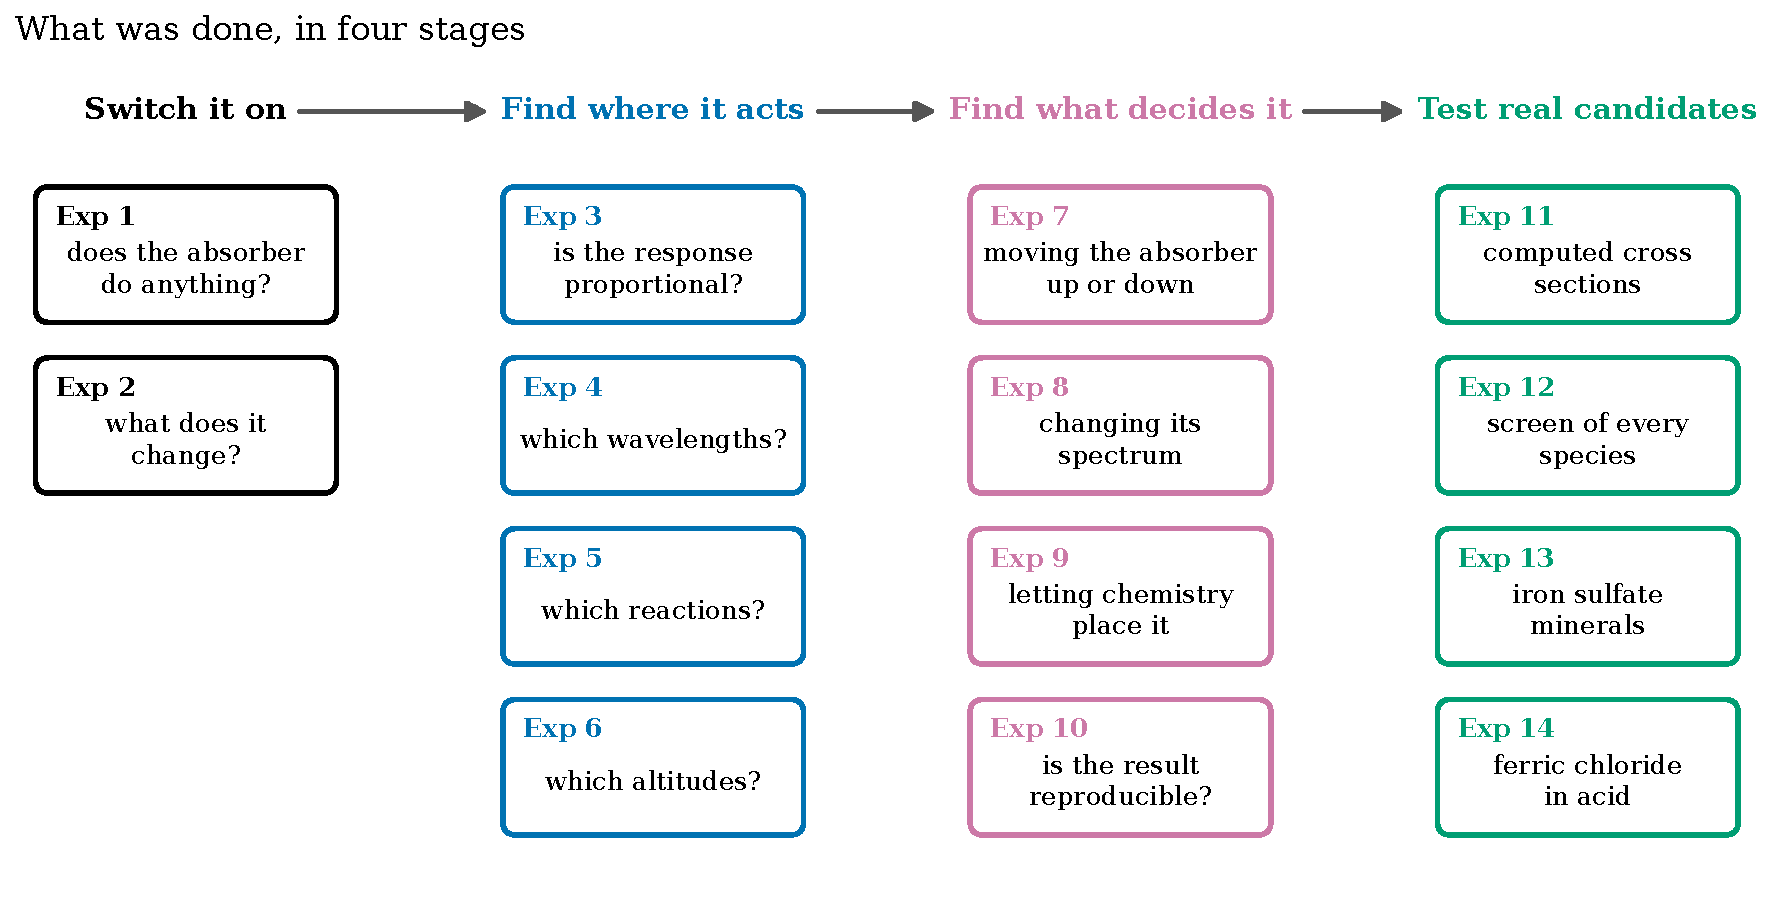
\includegraphics[width=\textwidth]{F04_CTX_what-was-done_ch3_report.pdf}
  \caption[What was done, in four stages]{What was done, in four stages. Each box is one experiment and the question it
    asked, and each stage builds on what the stage before it found. Source:
    \texttt{figures/scripts/F04\_CTX\_what-was-done.py}.}
  \label{fig:F4}
\end{figure}
